\documentclass[12pt]{report}
\usepackage[utf8]{inputenc}
\usepackage[russian]{babel}
\usepackage{setspace} % для междустрочного интервала
\onehalfspacing % 1.5 интервал между строками

\usepackage[left=30mm, top=20mm, right=20mm, bottom=20mm, nohead, footskip=7mm]{geometry}

\usepackage{titlesec, blindtext, color} 
\definecolor{gray75}{gray}{0.75}
\newcommand{\hsp}{\hspace{20pt}}
\titleformat{\chapter}[hang]{\Large\bfseries}{\thechapter{. }}{0pt}{\Large\bfseries}
\titlespacing{\chapter}{-5pt}{-30pt}{12pt} % отступ заголовка сверху
\titleformat{\section}[hang]{\large\bfseries}{\thesection{. }}{0pt}{\large\bfseries}

\makeatletter % список литературы
\def\@biblabel#1{#1. }
\makeatother

% Ссылки
\usepackage{hyperref}

% Возможность вставки pdf страниц
\usepackage{pdfpages}

% Листинги
\usepackage{listings}

% Для возможности переноса строк в equation, только надо еще и окружение \begin{gathered} сделать
\usepackage{amsmath}

\lstset{
	language = c++,
	extendedchars=\true,
	basicstyle=\small\sffamily,
	numbers=left,
	numberstyle=\tiny,
	stepnumber=1,
	numbersep=5pt,
	showspaces=false,            % показывать или нет пробелы специальными отступами
	showstringspaces=false,
	showtabs=false,
	frame=single,
	tabsize=2,
	captionpos=t,
	breaklines=true,
	breakatwhitespace=false,
	escapeinside={\#*}{*)},
	keepspaces=true
}

% Чтобы вместо : в подписях было -
\RequirePackage{caption}
\DeclareCaptionLabelSeparator{defffis}{ — }
\captionsetup{justification=centering,labelsep=defffis}

\usepackage{pgfplots}
\usepackage{pgfplotstable}
\pgfplotsset{compat=1.9}


\usepackage{csvsimple} %
\usepackage{datatool}




\begin{document}
	\renewcommand\bibname{Список литературы}
	
	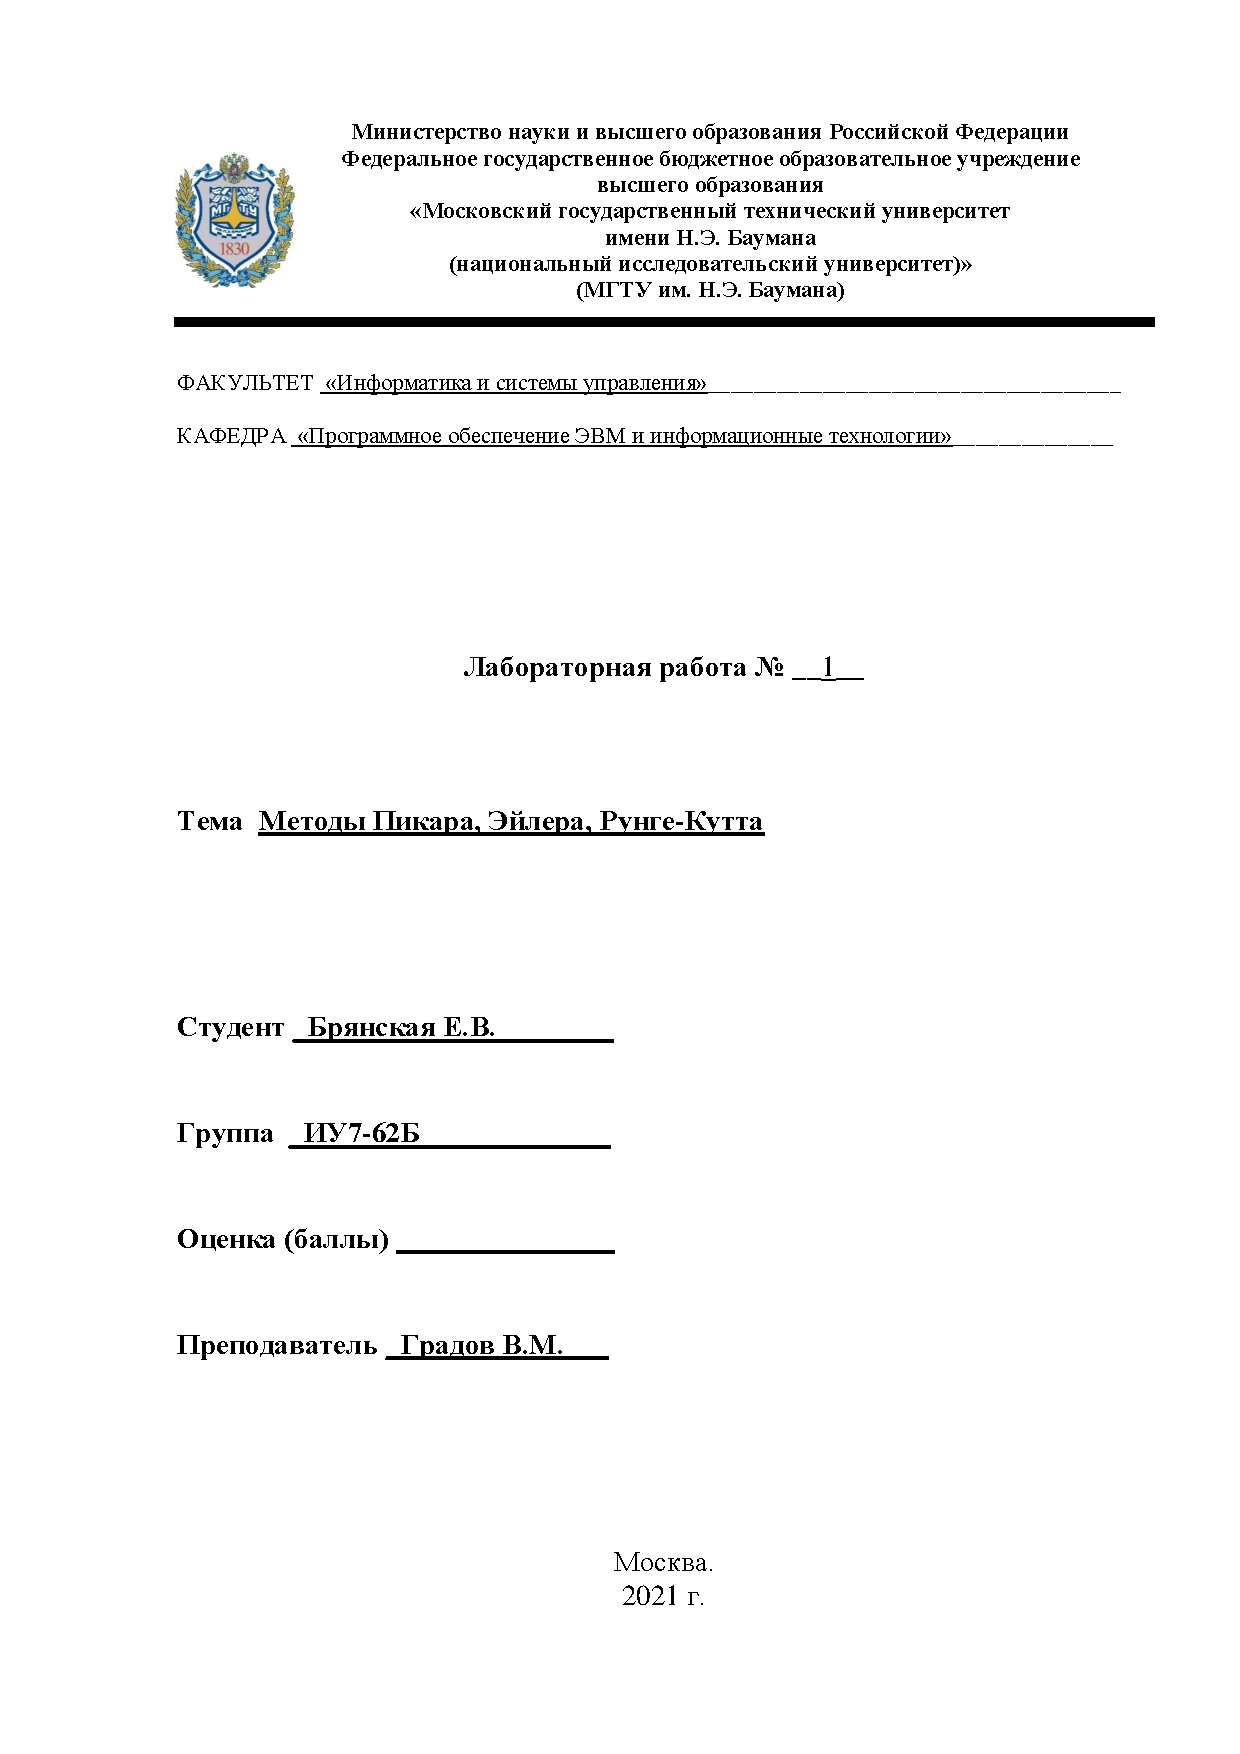
\includepdf[pages=1]{title.pdf}
	
	\newpage
	
	\chapter*{Выполнение}

Задача решается методом Рунге-Кутта 4ого порядка для системы ОДУ.\\
\begin{equation}
	y_{n + 1} = y_n + \frac{k_1 + 2k_2 + 2k_3 + k_4}{6},
	~~~~~~~~z_{n + 1} = z_n + \frac{p_1 + 2p_2 + 2p_3 + p_4}{6}
\end{equation}

где

\begin{equation}
	k_1 = hf(x_n, y_n, z_n)    
	~~~~~~~~p_1 = h\varphi(x_n, y_n, z_n)
\end{equation}

\begin{equation}
	k_2 = hf(x_n + \frac{h}{2}, y_n + \frac{k_1}{2}, z_n + \frac{p_1}{2})    
	~~~~~~~~p_2 = h\varphi(x_n + \frac{h}{2}, y_n + \frac{k_1}{2}, z_n + \frac{p_1}{2})
\end{equation}

\begin{equation}
	k_3 = hf(x_n + \frac{h}{2}, y_n + \frac{k_2}{2}, z_n + \frac{p_2}{2})    
	~~~~~~~~p_3 = h\varphi(x_n + \frac{h}{2}, y_n + \frac{k_2}{2}, z_n + \frac{p_2}{2})
\end{equation}

\begin{equation}
	k_4 = hf(x_n + \frac{h}{2}, y_n + k_3, z_n + p_3)    
	~~~~~~~~p_4 = h\varphi(x_n + \frac{h}{2}, y_n + k_3, z_n + p_3)
\end{equation}



	\subsection*{Приближённый аналитический метод Пикара}
\begin{equation}\label{formula4}
	\left\{
	\begin{array}{ccc}
		u'(x) = f(x, u),\\
		u(\xi) = \eta\\
	\end{array}
	\right.
\end{equation}

\begin{equation}\label{formula5}
	u(x) = \eta + \int\limits_\xi^x f(t, u(t))dt
\end{equation}

Получается, что
\begin{equation}\label{formula6}
	y^{(s)}(x) = \eta + \int\limits_\xi^x f(t, y^{(s - 1)}(t))dt
\end{equation}

\begin{equation}\label{formula7}
	y^{(0)} = \eta
\end{equation}

Найдём 1, 2, 3 и 4 приближение для (\ref{formula1}).\\
\begin{multline}\label{formula8}
	\shoveright
	{
		y^{(1)} = 0 + \int\limits_0^x t^2dt = \frac{t^3}{3}\bigg|_0^x = \frac{x^3}{3}
	}
\end{multline}


\begin{multline}\label{formula9}
	\shoveright
	{
		y^{(2)} = 0 + \int\limits_0^x [(\frac{t^3}{3})^2 + t^2]dt = \frac{t^7}{63}\bigg|_0^x + \frac{t^3}{3}\bigg|_0^x = \frac{x^7}{63} + \frac{x^3}{3}
	}
\end{multline}

\begin{multline}\label{formula10}
	\shoveright
	{
	\begin{gathered}
		y^{(3)} = 0 + \int\limits_0^x [(\frac{t^3}{3} + \frac{t^7}{63})^2 + t^2]dt = \frac{t^{15}}{15\cdot63^2}\bigg|_0^x + \frac{2\cdot t^{11}}{3\cdot63\cdot11}\bigg|_0^x + \frac{t^7}{63}\bigg|_0^x + \frac{t^3}{3}\bigg|_0^x = \\
		= \frac{x^{15}}{59535} + \frac{2\cdot x^{11}}{2079} + \frac{x^7}{63} + \frac{x^3}{3}
	\end{gathered}
	}
\end{multline}

\begin{multline}\label{formula11}
	\shoveright
	{
	\begin{gathered}
		y^{(4)} = 0 + \int\limits_0^x [(\frac{t^{15}}{59535} + \frac{2\cdot t^{11}}{2079} + \frac{t^7}{63} + \frac{t^3}{3})^2 + t^2]dt
		= \frac{x^{31}}{109 876 902 975} + \frac{4\cdot x^{27}}{3 341 878 155} + \\ + \frac{4\cdot x^{23}}{99 411 543} + \frac{2\cdot x^{23}}{86 266 215} + \frac{2\cdot x^{19}}{3 393 495} + \frac{4\cdot x^{19}}{2 488 563} + \frac{4\cdot x^{15}}{93 555} + \frac{x^{15}}{59 535} + \frac{2\cdot x^{11}}{2079} + \frac{x^7}{63} + \frac{x^3}{3}
	\end{gathered}
	}
\end{multline}

Реализация представлена на листинге \ref{code1}.\\







	\newpage
	
%	\chapter{Аналитическая часть}
	%\input{analytical_part.tex}
%	\newpage
	
	
%	\chapter*{Заключение}
%	\input{conclusion.tex}
%	\newpage
	
	\begin{thebibliography}{2}
		\addcontentsline{toc}{chapter}{Список литературы}
		\bibitem{Paral_methods}Иванов, К. К. Принципы разработки параллельных методов / К. К. Иванов, С. А. Раздобудько, Р. И. Ковалев. — Текст : непосредственный // Молодой ученый. — 2017. — № 3 (137). — С. 30-32. — URL: https://moluch.ru/archive/137/38412/ (дата обращения: 21.10.2020).
		\bibitem{Kormen} Кормен, Томас Х. и др Алгоритмы: построение и анализ, 3-е изд. : Пер. с англ. - М. : ООО "И.Д. Вильямс", 2018. - 1328 с. : ил. - Парал. тит. англ. -  ISBN 978-5-8459-2016-4 (рус.).
		\bibitem{thread} Документация по Стандартной библиотекн языка С++ thread [Электронный ресурс]. Режим доступа: https://docs.microsoft.com/ru-ru/cpp/standard-library/thread?view=vs-2019, свободный (дата обращения 22.10.2020)
		\bibitem{mutex} Документация по Стандартной библиотекн языка С++ mutex [Электронный ресурс]. Режим доступа: https://docs.microsoft.com/ru-ru/cpp/standard-library/mutex?view=vs-2019, свободный (дата обращения 22.10.2020)
		\bibitem{Visual} Документация по Visual Studio 2019 [Электронный ресурс]. Режим доступа: https://docs.microsoft.com/ru-ru/visualstudio/windows/?view=vs-2019, свободный (дата обращения: 21.10.2020)
		\bibitem{Query} QueryPerformanceCounter function [Электронный ресурс]. Режим доступа: https://docs.microsoft.com/en-us/windows/win32/api/profileapi/nf-profileapi-queryperformancecounter, свободный (дата обращения: 22.10.2020).
	\end{thebibliography}
\end{document}
